\documentclass[12pt,t]{beamer}
\usepackage{graphicx}
\usepackage[vlined]{algorithm2e}
\usepackage{times}
\usepackage{calc}
\usepackage{url}
\usepackage{soul}
\usepackage{graphicx}
\usepackage{multirow, hhline}
\usepackage{array, booktabs}
\usepackage{amsmath}
\usepackage{amssymb}
\usepackage{relsize}
\usepackage{multirow}
\usepackage{booktabs}
\usepackage{pagecolor}
\usepackage{lipsum}
\usepackage{capt-of}
\usepackage{booktabs}

\usepackage{graphicx}
\usepackage{multicol}
\usepackage[T1]{fontenc}
\usepackage{ae}
\graphicspath{{fig/}}
\setbeameroption{hide notes}
\setbeamertemplate{note page}[plain]

\usetheme{default}
\beamertemplatenavigationsymbolsempty
\hypersetup{pdfpagemode=UseNone}

\usefonttheme{professionalfonts}
\usefonttheme{serif}
\usepackage{fontspec}
\setmainfont{Karla}
\setbeamerfont{note page}{family*=pplx,size=\footnotesize} % Palatino for notes

\definecolor{foreground}{RGB}{70,70,70}
\definecolor{background}{RGB}{249, 249, 249} %24,24,24
%\definecolor{title}{RGB}{107,174,214} %107,174,214
\definecolor{title}{RGB}{70,70,70}
\definecolor{gray}{RGB}{0,0,0}
\definecolor{subtitle}{RGB}{70,70,70}
\definecolor{hilight}{RGB}{102,255,204}
\definecolor{vhilight}{RGB}{255,111,207}

\setbeamercolor{titlelike}{fg=title}
\setbeamercolor{subtitle}{fg=subtitle}
\setbeamercolor{institute}{fg=gray}
\setbeamercolor{normal text}{fg=foreground,bg=background}


\setbeamercolor{item}{fg=foreground} % color of bullets
\setbeamercolor{subitem}{fg=gray}
\setbeamercolor{itemize/enumerate subbody}{fg=gray}
\setbeamertemplate{itemize subitem}{{\textendash}}
\setbeamerfont{itemize/enumerate subbody}{size=\footnotesize}
\setbeamerfont{itemize/enumerate subitem}{size=\footnotesize}

\setbeamercolor{block title}{fg=white,bg=gray!70}
\setbeamercolor{block body}{fg=black,bg=gray!10}
\setbeamercolor{block title alerted}{fg=red,bg=gray!40}
\setbeamercolor{block title example}{fg=black,bg=green!20}
\setbeamercolor{block body example}{fg=black,bg=green!5}
\setbeamerfont{block title}{series=\bfseries}

\hypersetup{colorlinks,linkcolor=foreground,urlcolor=foreground}


\setbeamertemplate{footline}{%
    \raisebox{5pt}{\makebox[\paperwidth]{\hfill\makebox[20pt]{\color{gray}
          \scriptsize\insertframenumber}}}\hspace*{5pt}}

\addtobeamertemplate{note page}{\setlength{\parskip}{12pt}}


\newcommand{\bi}{\begin{itemize}}
\newcommand{\ei}{\end{itemize}}
\newcommand{\ig}{\includegraphics}
\newcommand{\subt}[1]{{\footnotesize \color{subtitle} {#1}}}

\let\emph\relax % there's no \RedeclareTextFontCommand
\DeclareTextFontCommand{\emph}{\bfseries\em}


\setbeamertemplate{frametitle}
{\vskip4pt
  \leavevmode
%\hbox{%
\begin{beamercolorbox}[wd=\paperwidth,ht=2ex,dp=0ex]{frametitle}%
\underline{\makebox[\paperwidth][l]{\hspace*{10pt}
\large {{\insertframetitle}}}}
\end{beamercolorbox}
%  }%
}

%\setbeamercolor{frametitle}{fg=yellow,bg=red}

\begin{document}

\AtBeginSection[]{
  \begin{frame}
  \vfill
  \centering
  \begin{beamercolorbox}[sep=8pt,center,shadow=true,rounded=true]{title}
    \underline{\makebox[0.6\paperwidth][l]{
\large {{\insertsectionhead}}}}
  \end{beamercolorbox}
  \vfill
  \end{frame}
}

\title{\large{Lecture \#2: Introduction to Regression}}
\subtitle{CS 109A, STAT 121A, AC 209A: Data Science}
\author{Pavlos Protopapas \and Kevin Rader}
%\institute{Harvard University}
\date{}
\titlegraphic{
   
\includegraphics[height=2cm]{iacs}
\includegraphics[height=2cm]{hogwarts}
}
{
\setbeamertemplate{footline}{} % no page number here
\frame{
  \titlepage
  
}
}


\begin{frame}{Lecture Outline}
\tableofcontents
\end{frame}

%%%%%%%%%%%%%%%%%%%%%%%%%%%%%%%%%%%%%%%%%%%%%%%%%%%%%%%%%%%%%%%%%%%%%%%%%%%%%%
\section{Statistical Modeling}

%%%%%%%%%%%%%%
\begin{frame}{Predicting a Variable} 
Let's image a scenario where we'd like to predict one variable using another (or a set of other) variables.
\vskip0.2cm
\textbf{Examples:}
\begin{itemize}
\setlength{\itemsep}{0.4cm}
\item Predicting the amount of view a YouTube video will get next week based on video length, the date it was posted, previous number of views, etc.
\item Predicting which movies a Netflix user will rate highly based on their previous movie ratings, demographic data etc.
\item Predicting the expected cab fare in New York City based on time of year, location of pickup, weather conditions etc.
\end{itemize}
\end{frame}

%%%%%%%%%%%%%%
\begin{frame}{Outcome vs. Predictor Variables} 
\only<1>{
There is an asymmetry in many of these problems: the variable we'd like to predict may be more difficult to measure, is more important than the other(s), or may be directly or indirectly influenced by the values of the other variable(s). 
\vskip0.5cm
Thus, we'd like to define two categories of variables: variables whose value we want to predict and variables whose values we use to make our prediction.
}
\only<2>{
\vskip-0.5cm
\begin{block}{Definition}
Suppose we are observing $p + 1$ number variables and we are making $n$ sets observations. We call
\begin{itemize}
\item the variable we'd like to predict the \emph{outcome} or \emph{response variable}; typically, we denote this variable by $Y$ and the individual measurements $y_i$.
\vskip0.2cm
\item the variables we use in making the predictions the \emph{features} or \emph{predictor variables}; typically, we denote these variables by $X=(X_1,\ldots, X_p)$ and the individual measurements $x_{i, j}$.
\end{itemize}
\end{block}
\textbf{Note:} $i$ indexes the observation ($i = 1, 2, \ldots, n$) and $j$ indexes the value of the $j$-th predictor variable ($j = 1, 2, \ldots, p$).
}
\end{frame}

%%%%%%%%%%%%%%
\begin{frame}{True vs. Statistical Model} 
We will assume that the response variable, $Y$, relates to the predictors, $X$, through some unknown function expressed generally as:
\[
Y = f(X) + \epsilon.
\]
Here, 
\begin{itemize}
\item $f$ is the unknown function expressing an underlying rule for relating $Y$ to $X$, 
\item $\epsilon$ is random amount (unrelated to $X$) that $Y$ differs from the rule $f(X)$
\end{itemize}
\vskip0.2cm
A \emph{statistical model} is any algorithm that estimates $f$. We denote the estimated function as $\widehat{f}$.
\end{frame}

%%%%%%%%%%%%%%
\begin{frame}{Prediction vs. Estimation} 
\vskip-0.4cm
For some problems, what's important is obtaining $\widehat{f}$, our estimate of $f$. These are called \emph{inference} problems. 
\vskip0.2cm
When we use a set of measurements of predictors, $(x_{i, 1}, \ldots, x_{i, p})$, in an observation to predict a value for the response variable, we denote the \emph{predicted value} by $\widehat{y}_i$,
\[
\widehat{y}_i = \widehat{f}(x_{i, 1}, \ldots, x_{i, p}).
\]
For some problems, we don't care about the specific form $\widehat{f}$, we just want to make our prediction $\widehat{y}_i$ as close to the observed value $y_i$ as possible. These are called \emph{prediction problems}.
\vskip0.2cm
We'll see that some algorithms are better suited for inference and others for prediction.
\end{frame}

%%%%%%%%%%%%%%%%%%%%%%%%%%%%%%%%%%%%%%%%%%%%%%%%%%%%%%%%%%%%%%%%%%%%%%%%%%%%%%
\section{Regression vs. Classification}

%%%%%%%%%%%%%%
\begin{frame}{Outcome Variables} 
\vskip-0.4cm
There are two main types of prediction problems we will see this semester:
\vskip0.2cm
\begin{itemize}
\item \emph{Regression problems} are ones with a quantitative response variable.\\

\textbf{Example}: Predicting the number of taxicab pick-ups in New York.
\vskip0.2cm
\item \emph{Classification problems} are ones with a categorical response variable.\\

\textbf{Example}: Predicting whether or not a Netflix user will like a particular movie.
\end{itemize}
\vskip0.2cm
This distinction is important, as each type of problem may require it's own specialized algorithms along with metrics measuring effectiveness.
\end{frame}

%%%%%%%%%%%%%%%%%%%%%%%%%%%%%%%%%%%%%%%%%%%%%%%%%%%%%%%%%%%%%%%%%%%%%%%%%%%%%%
\section{Error, Loss Functions}

%%%%%%%%%%%%%%
\begin{frame}{Error \& Loss Functions} 
\vskip-0.4cm
In order to quantify how well a model performs, we define a \emph{loss} or \emph{error function}.
\vskip0.2cm
A common loss function for quantitative outcomes is the \emph{Mean Squared Error (MSE)}:
\[
MSE = \frac{1}{n}\sum_{i=1}^n (y_i - \widehat{y}_i)^2
\]
The quantity $|y_i - \widehat{y}_i|$ is called a \emph{residual} and measures the error at the $i$-th prediction.
\vskip0.2cm
\textbf{Caution:} The MSE is by no means the only valid (or the best) loss function!
\vskip0.2cm
\textbf{Question:} What would be an intuitive loss function for predicting categorical outcomes? 
\end{frame}

%%%%%%%%%%%%%%
\begin{frame}{Using Loss Functions} 
Loss functions are used to choose a suitable estimate $\widehat{f}$ of $f$. 
\vskip0.2cm
A statistical modeling approach is often an algorithm that:
\begin{itemize}
\item assumes some mathematical form for $f$, and hence for $\widehat{f}$,
\item then chooses values for the unknown parameters of $\widehat{f}$ so that the loss function is minimized on the set of observations
\end{itemize}
\end{frame}

%%%%%%%%%%%%%%
\begin{frame}{Line of Best Fit} 
Which of the following linear models is the best? How do you know?
\begin{center}
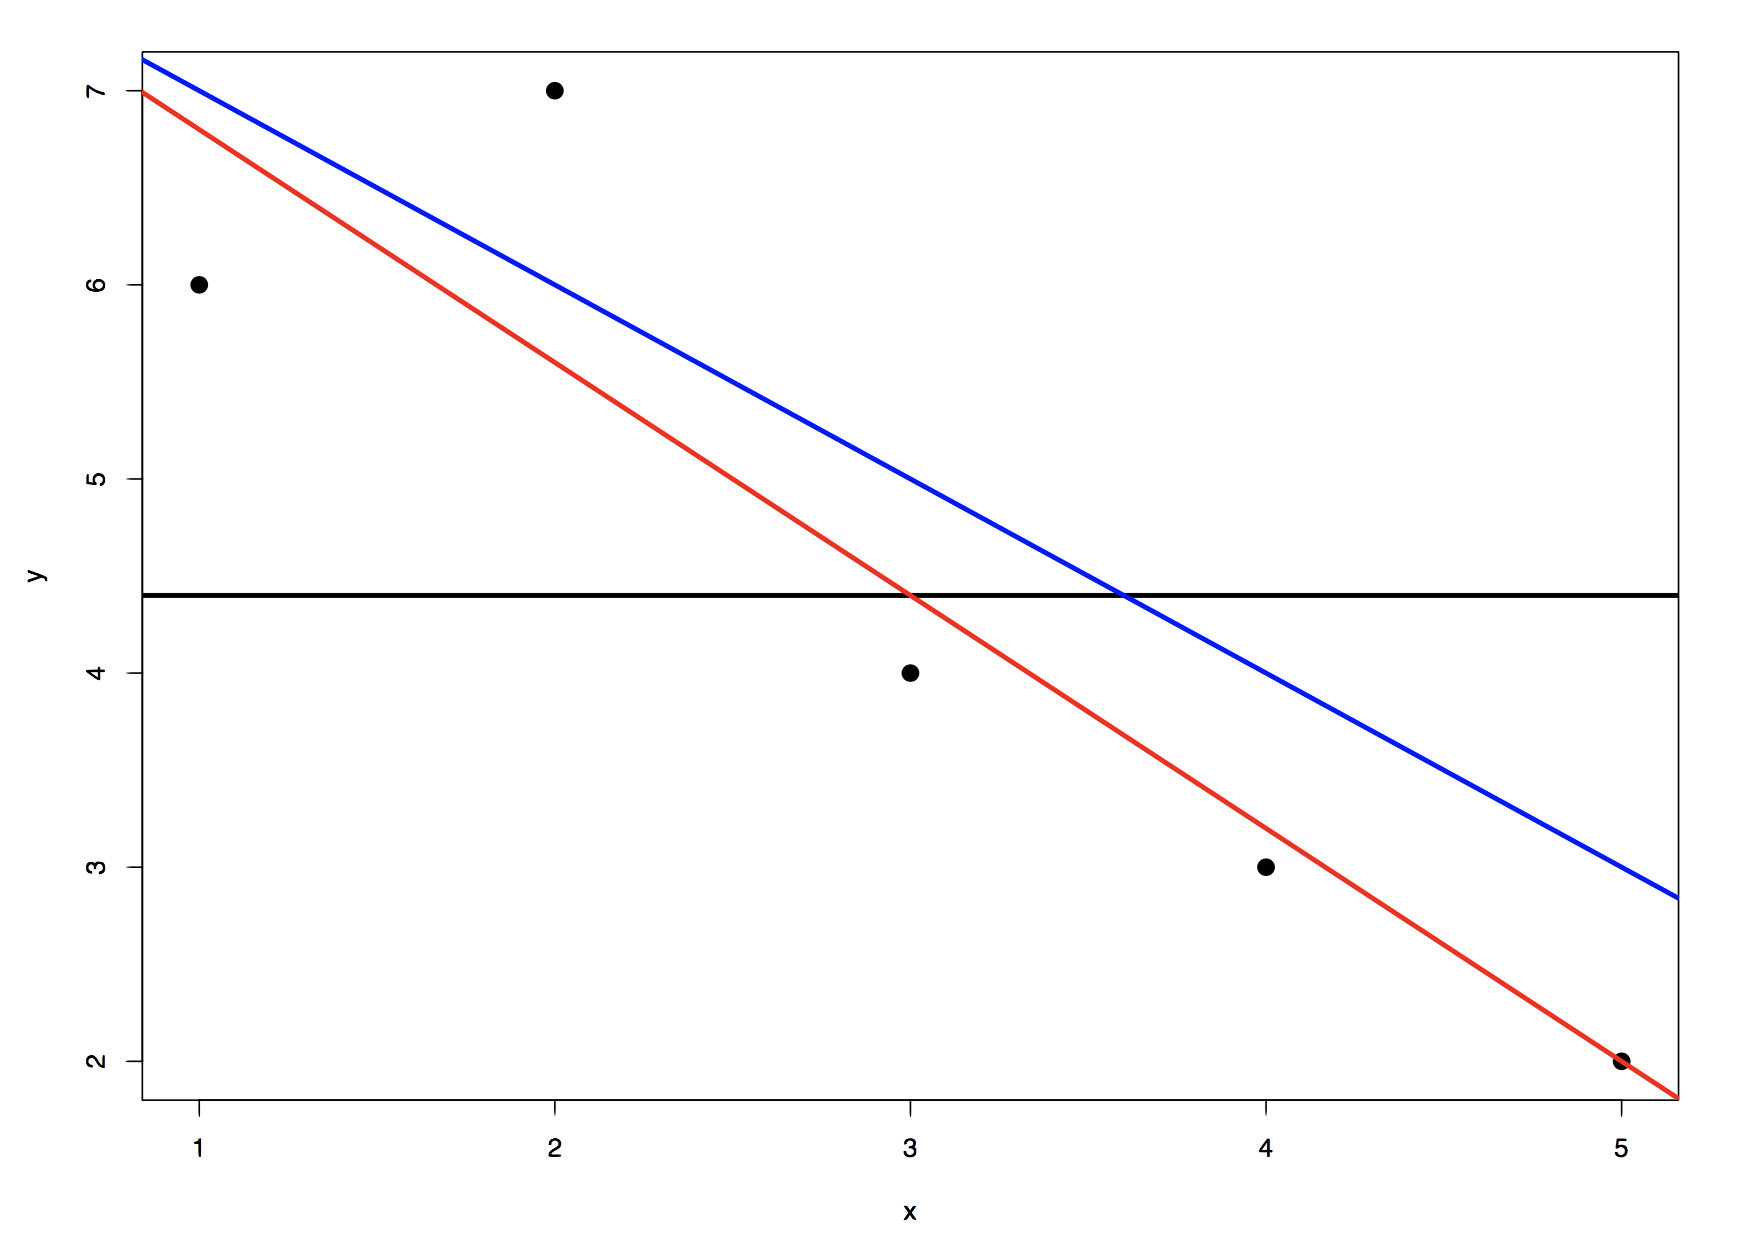
\includegraphics[width=80mm]{lecture2_g1}
\end{center}
\end{frame}


%%%%%%%%%%%%%%%%%%%%%%%%%%%%%%%%%%%%%%%%%%%%%%%%%%%%%%%%%%%%%%%%%%%%%%%%%%%%%%
\section{Model I: k-Nearest Neighbours}

%%%%%%%%%%%%%%
\begin{frame}{k-Nearest Neighbours} 
\only<1>{
The \emph{$k$-Nearest Neighbour (kNN) model} is a intuitive way to predict an quantitative response variable: 
\vskip0.2cm
\begin{quote}
to predict a response for a set of observed predictor values, we use the responses of other observations most similar to it!
\end{quote}
\vskip0.2cm
\textbf{Note:} this strategy can also be applied in classification to predict a categorical variable. We will encounter kNN again later in the semester in the context of classification.
}
\only<2>{
\begin{block}{k-Nearest Neighbours}
Fixed a value of $k$. The predicted response for the $i$-th observation is the average of the observed response of the $k$-closest observations 
\[
\widehat{y}_i = \frac{1}{k} \sum_{i=1}^k y_{n_i}
\]
where $\{ X_{n_1}, \ldots, X_{n_k}\}$ are the $k$ observations most similar to $X_i$ (``similar" refers to a notion of distance between predictors).
\end{block}
}
\end{frame}

%%%%%%%%%%%%%%
\begin{frame}{kNN Regression: A Simple Example} 
\only<1-4>{
\vskip-0.4cm
Suppose you have 5 observations of taxi cab pick ups in New York City, the response is the average cab fare (in units of \$10), and the predictor is time of day (in hours after 7am):
\begin{center}
\begin{tabular}{r | l l l l l}
$X$ & 1 & 2 & 3 & 4 & 5\\
\hline
$Y$ & 6 & 7 & 4 & 3 & 2\\
\end{tabular}
\end{center}
We calculate the predicted number of pickups using kNN for $k=2$:
\[
\only<1>{
\widehat{y}_1 = \frac{1}{2}\left( 7 + 4\right) = 5.5
}
\only<2>{
\widehat{y}_2 = \frac{1}{2}\left( 6 + 4\right) = 5.0
}
\only<3->{
\widehat{Y} = (5.5, 5.0, 5.0, 3.0, 3.5)
}
\]
\only<4>{
The MSE given our predictions is
\[
MSE = \frac{1}{5} \left[ (6 - 5.5)^2 + (7 - 5.0)^2 + \ldots + (3.5 - 2)^2\right] = 1.5
\]
On average, our predicts are off by 150 pickups.
}
}
\only<5>{
\vskip-0.4cm
We plot the observed responses along with predicted responses for comparison:
\begin{center}
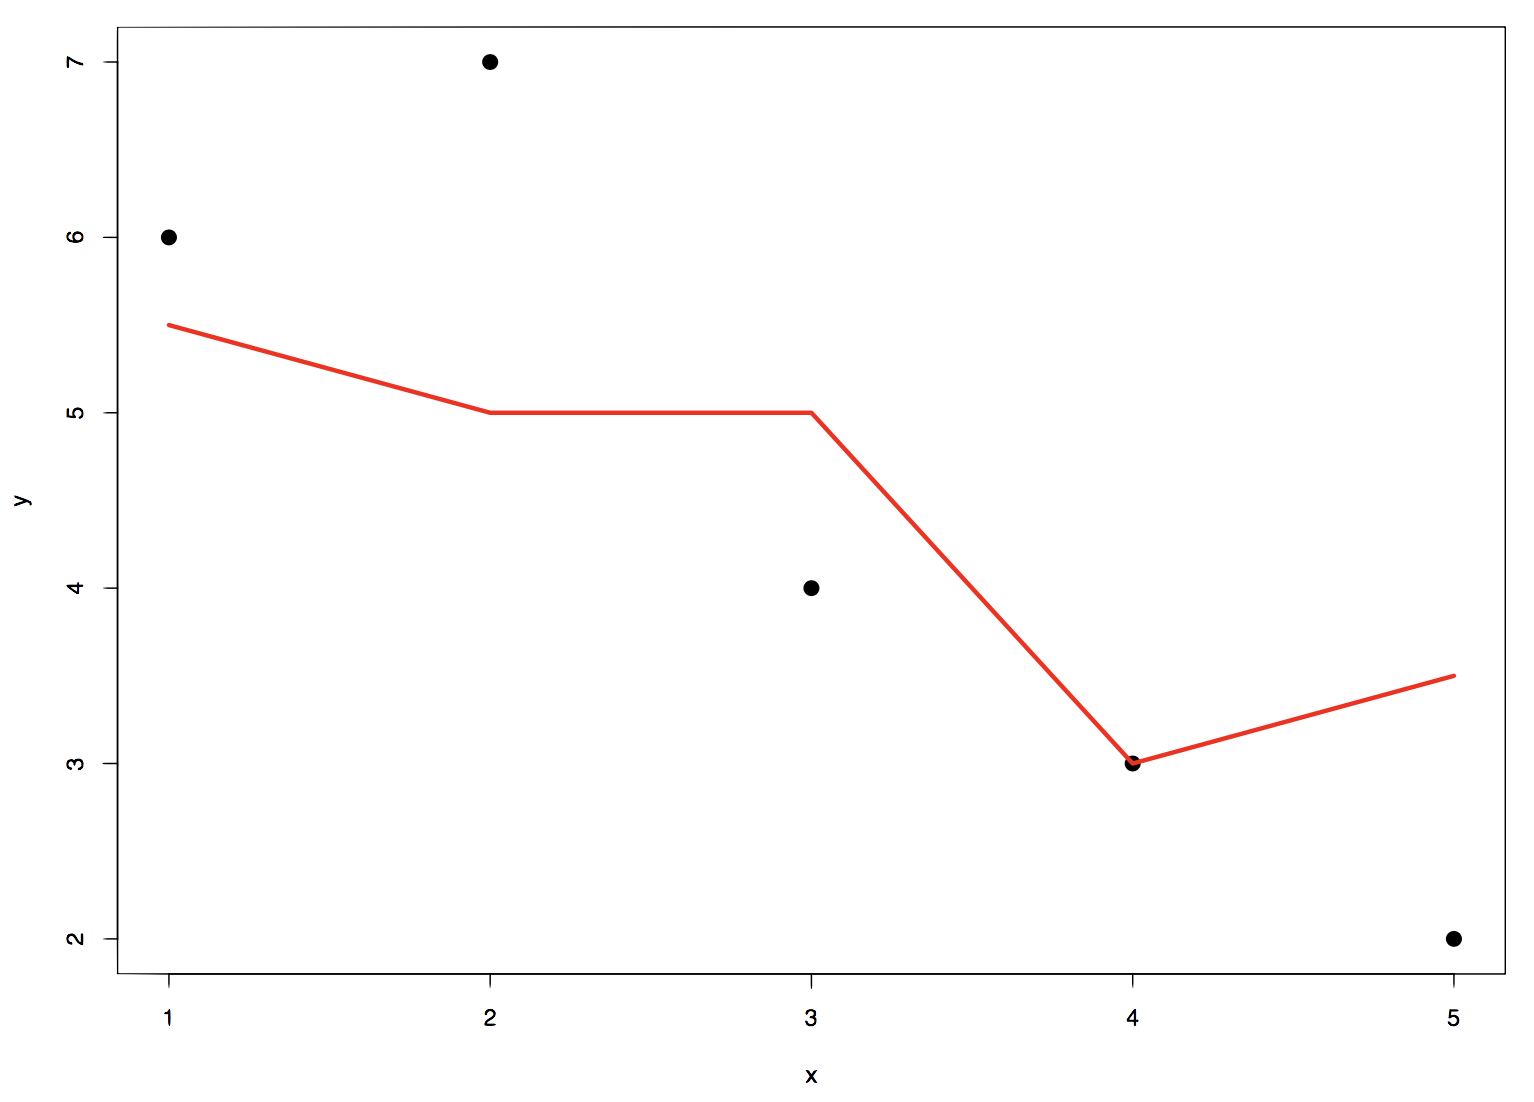
\includegraphics[width=90mm]{lecture2_g2}
\end{center}
}
\end{frame}

%%%%%%%%%%%%%%
\begin{frame}{Choice of k Matters} 
\vskip-0.4cm
But what value of $k$ should we choose? What would our predicted responses look like if $k$ is very small? What if $k$ is large (e.g. $k = n$)?
\begin{center}
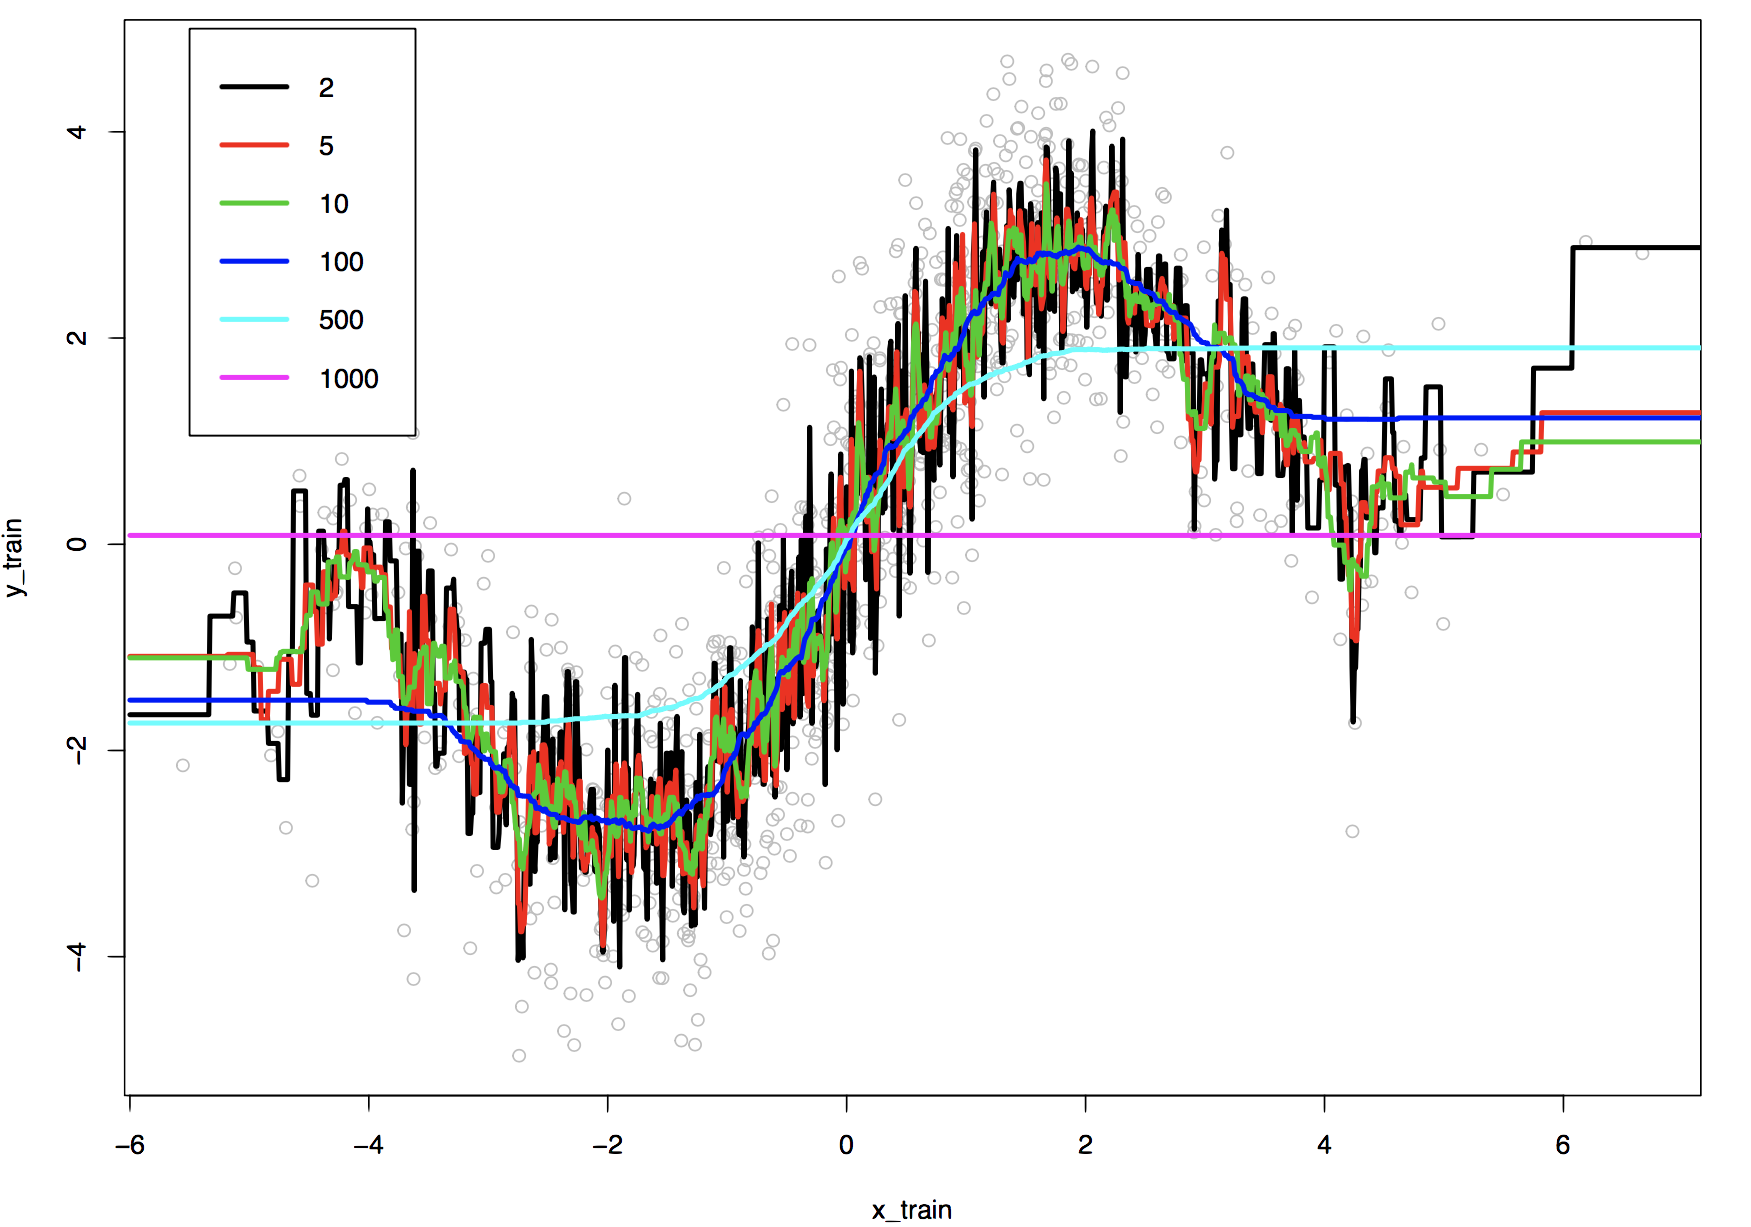
\includegraphics[width=90mm]{lecture2_g3}
\end{center}
\end{frame}


%%%%%%%%%%%%%%
\begin{frame}{kNN with Multiple Predictors} 
In our simple example, we used absolute value to measure the distance between the predictors in two different observations, $|x_i - x_j|$. 
\vskip0.2cm
When we have multiple predictors in each observation, we need a notion of distance between two \textbf{sets} of predictor values. Typically, we use Euclidean distance:
\[
d(x_i - x_j) = \sqrt{(x_{i, 1} - x_{j, 1})^2 + \ldots + (x_{i, p} - x_{j, p})^2}
\]
\textbf{Caution:} when using Euclidean distance, the scale (or units) of measurement for the predictors matter! Predictors with large values, comparatively, will dominate the distance measurement.
\end{frame}


%%%%%%%%%%%%%%%%%%%%%%%%%%%%%%%%%%%%%%%%%%%%%%%%%%%%%%%%%%%%%%%%%%%%%%%%%%%%%%
\section{Model II: Linear Regression}

%%%%%%%%%%%%%%
\begin{frame}{Linear Models in One Variable} 
Note that in building our kNN model for prediction, we did not compute a closed form for $\widehat{f}$, our estimate of the function, $f$, relating predictor to response. 
\vskip0.4cm
Alternatively, if each observation has only one predictor, we can build a model by first assuming a simple form for $f$ (and hence $\widehat{f}$), say a \emph{linear form}, 
\[
Y = f(X) + \epsilon = \beta_1 X + \beta_0 + \epsilon.
\]
Again, $\epsilon$ is the random quantity or \emph{noise} by which observed values of $Y$ differ from the rule $f(X)$. 
\end{frame}

%%%%%%%%%%%%%%
\begin{frame}{Inference for Linear Regression} 
\only<1>{
If our statistical model is 
\[
Y = f(X) + \epsilon = \beta^{\text{true}}_1 X + \beta^{\text{true}}_0 + \epsilon,
\]
then it follows that our estimate is
\[
\widehat{Y} = \widehat{f}(X) = \widehat{\beta_1} X +\widehat{\beta_0}
\]
where $\widehat{\beta_1}$ and $\widehat{\beta_0}$ are estimates of $\beta_1$ and $\beta_0$, respectively, that we compute using observations.
\vskip0.4cm
Recall that our intuition says to choose $\widehat{\beta_1}$ and $\widehat{\beta_0}$ in order to minimize the predictive errors made by our model, i.e. minimize our loss function.
}
\only<2>{
\vskip-0.4cm
Again we use MSE as our loss function,
\[
L(\beta_0, \beta_1) = \frac{1}{n}\sum_{i=1}^n \left(y_i - \widehat{y}_i \right)^2 = \frac{1}{n}\sum_{i=1}^n \left[y_i - (\beta_1 X + \beta_0) \right]^2.
\]
Then the optimal values for $\widehat{\beta_1}$ and $\widehat{\beta_0}$ should be 
\[
\widehat{\beta}_0, \widehat{\beta}_1 = \underset{\beta_0, \beta_1}{\mathrm{argmin}}L(\beta_0, \beta_1).
\]
Now, taking the partial derivatives of $L$ and finding the global minimum will give us explicit formulae for $\widehat{\beta}_0, \widehat{\beta}_1$,
\begin{align*}
\widehat{\beta}_1 &= \frac{\sum_i (x_i - \overline{x})(y_i - \overline{y})}{\sum_i (x_i - \overline{x})^2},  &\widehat{\beta}_0 &= \overline{y} - \widehat{\beta}_1 \overline{x}
\end{align*}
where $\overline{y}$ and $\overline{x}$ are sample means. The line $\widehat{Y} =  \widehat{\beta_1} X +\widehat{\beta_0}$ is called the \emph{regression line}.
}
\end{frame}

%%%%%%%%%%%%%%
\begin{frame}{Linear Regression: A Simple Example} 
\only<1>{
\vskip-0.4cm
Recall our simple example from before, where we observe the average cab fare in NYC using the time of day,
\begin{center}
\begin{tabular}{r | l l l l l}
$X$ & 1 & 2 & 3 & 4 & 5\\
\hline
$Y$ & 6 & 7 & 4 & 3 & 2\\
\end{tabular}
\end{center}
By our formula, we compute the regression line to be
\[
\widehat{Y} = -1.2X + 8
\]
Using this model, we can generate predicted responses:
\[
\widehat{Y} = (6.8, 5.6, 4.4, 3.2, 2.0)
\]
Let's graph our linear model against the observations.
}
\only<2>{
\begin{center}
\vskip-1cm
\begin{tabular}[t]{m{40mm}m{6cm}}
\multicolumn{1}{m{6cm}}{Why doesn't our line fit the observations exactly? There are two possibilities:
\begin{itemize}
\item $f$ is not a linear function
\item the difference between prediction and observation is due to the noise term in $Y = f(X) + \epsilon$.
\end{itemize}
} & 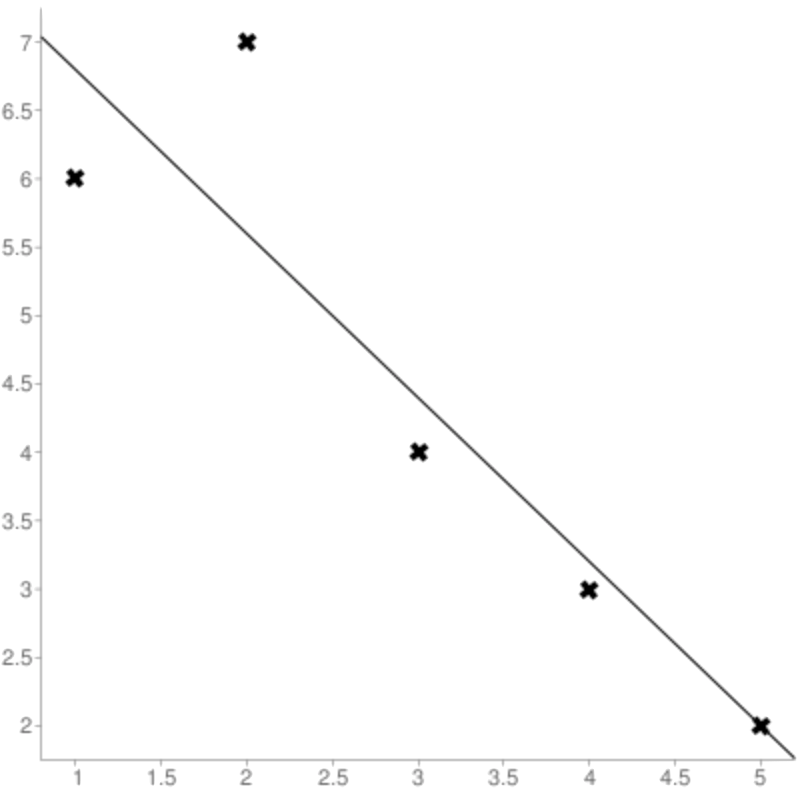
\includegraphics[width=40mm]{lecture2_g4}
\end{tabular}
\end{center}
\vskip-0.4cm
Regardless of the form of $f$, the presence of the random term $\epsilon$ means that the predictions made using $\widehat{f}$ will never exactly match the observations.
\vskip0.2cm
\textbf{Question: } Is it possible to measure how confidently $\widehat{\beta}_0$,  $\widehat{\beta}_1$ approximate the true parameters of $f$?
}
\end{frame}

\section{Evaluating Model Performance}

%%%%%%%%%%%%%%
\begin{frame}{Measurement vs. Sampling Error} 
\only<1>{
We interpret the $\epsilon$ term in our observation 
\[
Y = f(X) + \epsilon
\] 
to be noise introduced by random variations in natural systems or imprecisions of our scientific instruments. 
\vskip0.2cm
We call $\epsilon$ the measurement error or \emph{irreducible error}. Since even predictions made with the actual function $f$ will not match observed values of $Y$.
\vskip0.2cm
Due to $\epsilon$, every time we measure the response $Y$ for a fix value of $X$ we will obtain a different observation, and hence a different estimate of $\beta_0$ and $\beta_1$. 
}
\only<2>{
Again due to $\epsilon$, if we make only a few observations, the noise in the observed values of $Y$ will have a large impact on our estimate of $\beta_0$ and $\beta_1$. 
\vskip0.2cm
If we make many observations, the noise in the observed values of $Y$ will `cancel out' - noise that bias some observations towards higher values will be canceled with noise that bias other observations towards lower values. 
\vskip0.2cm
This feels intuitively true but requires some assumptions on $\epsilon$ and a formal justification - or at least an example.
}
\only<3>{
In summary, the variations in $\widehat{\beta}_0$,  $\widehat{\beta}_1$ (estimates of $\beta_0$ and $\beta_1$ respectively) are affected by
\vskip0.2cm
\begin{itemize}
\item (\textbf{Measurement}) $\mathrm{Var}[\epsilon]$, the variance (the scale of the variation) in the noise, $\epsilon$ 
\vskip0.4cm
\item (\textbf{Sampling}) $n$, the number of observation we make
\end{itemize}
\vskip0.2cm
The variances of $\widehat{\beta}_0$,  $\widehat{\beta}_1$ are also called \emph{standard errors}. 
}
\end{frame}

%%%%%%%%%%%%%%
\begin{frame}{Bootstrapping for Estimating Sampling Error}
\vskip-0.4cm
With some assumption on $\epsilon$, we can compute the variances or standard errors of $\widehat{\beta}_0$ and $\widehat{\beta}_1$ analytically. 
\vskip0.2cm
The standard errors can also be estimated empirically through \emph{bootstrapping}.
\vskip0.2cm
\begin{block}{Definition}
Bootstrapping is the practice of estimating properties of an estimator by measuring those properties by, for example, sampling from the observed data.
\end{block}
\vskip0.2cm
For example, we can compute $\widehat{\beta}_0$ and $\widehat{\beta}_1$ multiple times by randomly sampling from our data set. We then use the variance of our multiple estimates to approximate the true variance of $\widehat{\beta}_0$ and $\widehat{\beta}_1$.
\end{frame}

%%%%%%%%%%%%%%
\begin{frame}{Training vs. Testing Sets} 
One more way to evaluate our model is to use it to predict the responses for predictors that we did not use to build our model.
\vskip0.2cm
Typically, after collecting a set of observations of predictor and response, we split the data into a \emph{training set} and a \emph{testing set}. 
\vskip0.2cm
We use the training set to build a model and use the testing set to perform a final evaluation of the model, simulating model performance in real-time usage.
\vskip0.2cm
\textbf{Caution:} In order to maintain the integrity of the final test, you should use your test data one once and must not use the results to inform changes you make to the model.
\end{frame}

%%%%%%%%%%%%%%%%%%%%%%%%%%%%%%%%%%%%%%%%%%%%%%%%%%%%%%%%%%%%%%%%%%%%%%%%%%%%%%
\section{Comparison of Two Models}

%%%%%%%%%%%%%%
\begin{frame}{Parametric vs. Non-parametric Models} 
Linear regression is an example of \emph{a parametric model}, that is, it is a model with a fixed form and a fixed number of parameters that does not depend on the number of observations in the training set.
\vskip0.4cm
kNN is an example of a \emph{non-parametric model}, that is, it is a model whose structure depends on the data. The set of parameters of the kNN model is the entire training set.
\vskip0.2cm
In particular, the number of parameters in kNN depends on the number of observations in the training set.
\end{frame}

%%%%%%%%%%%%%%
\begin{frame}{kNN vs. Linear Regression} 
So which model is better? Rather than answer this question, let's define `better'. 
\vskip0.2cm
To compare two models, we can consider any combination of the following criteria (and possibly more): 
\vskip0.2cm
\begin{itemize}
\item Which model gives less predictive error, with respect to a loss function?
\vskip0.2cm
\item Which model takes less space to store?
\vskip0.2cm
\item Which model takes less time to train (perform inference)?
\vskip0.2cm
\item Which model takes less time to make a prediction?
\end{itemize}
\end{frame}


%%%%%%%%%%%%%%%%%%%%%%%%%%%%%%%%%%%%%%%%%%%%%%%%%%%%%%%%%%%%%%%%%%%%%%%%%%%%%%
\begin{frame}{Bibliography}

\begin{enumerate}
 \fontsize{8}{10}\selectfont
\item Bolelli, L., Ertekin, S., and Giles, C. L. \emph{Topic and trend detection in text collections using latent dirichlet allocation}. In European Conference on Information Retrieval (2009), Springer, pp. 776-780.
\item Chen, W., Wang, Y., and Yang, S. \emph{Efficient influence maximization in social networks. In Proceedings of the 15th ACM SIGKDD international conference on Knowledge discovery and data mining (2009)}, ACM, pp. 199-208.
\item Chong, W., Blei, D., and Li, F.-F. \emph{Simultaneous image classification and annotation. In Computer Vision and Pattern Recognition}, 2009. CVPR 2009. IEEE Conference on (2009), IEEE, pp. 1903-1910.
\item Du, L., Ren, L., Carin, L., and Dunson, D. B. \emph{A bayesian model for simultaneous image clustering, annotation and object segmentation}. In Advances in neural information processing systems (2009), pp. 486-494.
\item Elango, P. K., and Jayaraman, K. \emph{Clustering images using the latent dirichlet allocation model.}
\item Feng, Y., and Lapata, M. \emph{Topic models for image annotation and text illustration}. In Human Language Technologies: The 2010 Annual Conference of the North American Chapter of the Association for Computational Linguistics (2010), Association for Computational Linguistics, pp. 831-839.
\item Hannah, L. A., and Wallach, H. M. \emph{Summarizing topics: From word lists to phrases.}
\item Lu, R., and Yang, Q. \emph{Trend analysis of news topics on twitter}. International Journal of Machine Learning and Computing 2, 3 (2012), 327.
\end{enumerate}

\end{frame}

\end{document}
